%%% -*- mode:latex; mode:flyspell -*-

%%% Local Variables:
%%% TeX-master: "mu2e-36575"
%%% End:
\section{Tuning the calorimeter timing resolution}

The calorimeter timing has been tuned as shown in Figure \ref{fig:calorimeter_timing_resolution_2batch}.

{\red Stefano to add }

\begin{figure}[h]
  \hspace{-0.6in}
  \begin{tikzpicture}
    \node[anchor=south west,inner sep=0] at (-1,0.) {
      % \node[shift={(0 cm,0.cm)},inner sep=0,rotate={90}] at (0,0) {}
      \makebox[\textwidth][c] {
        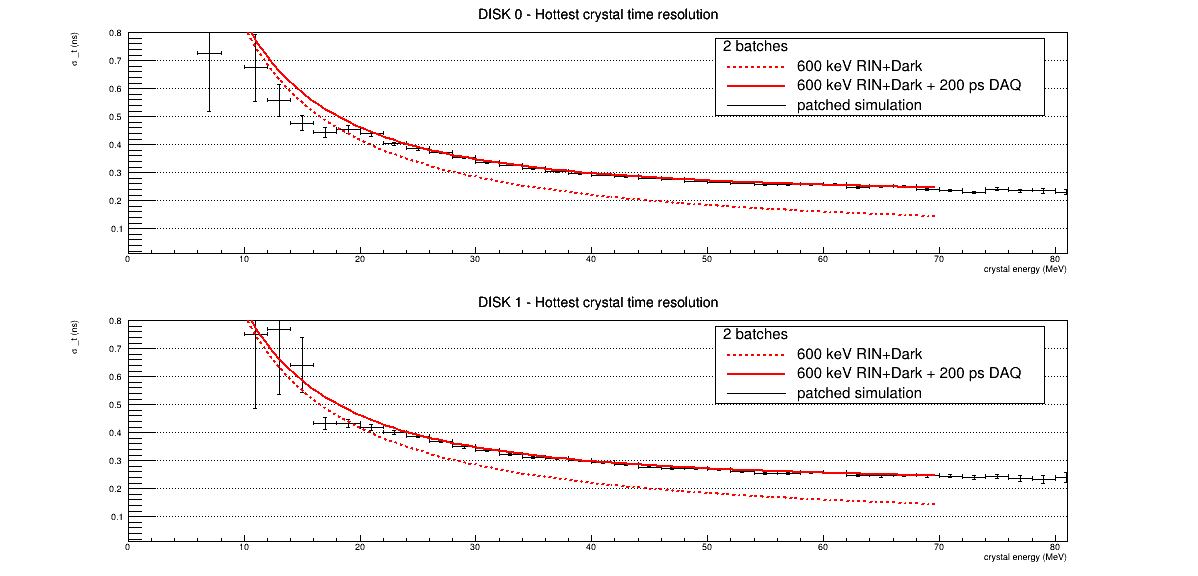
\includegraphics[width=0.80\textwidth]{figures/png/calorimeter_timing_2batch}
      }
    };
    % \node [text width=6cm, scale=0.8] at (4.5,6.4) {mu2e-18894 by Kevin Lynch and Jim Popp};
  \end{tikzpicture}
  % \captionof{figure} {
  \caption{
    \label{fig:calorimeter_timing_resolution_2batch}
    Tuned calorimeter timing resolution 
  }
\end{figure}

The resolution tuning has been performed after the global track-to-calorimeter timing offsets
have been corrected. The global correction introduced was 1.86ns, while after the tuning, the offset
value is about 1.6 ns. Resulting non-accounted for systematic offset of about 0.25 ns is however
about x2 smaller than the offset introduced by the Kalman fitter. 